%%%%%%%%%%%%%%%%%%%%%%%%%%%%%%%%%%%%%%%%%%%%%%%%%%%%%%%%%%%%%%%%%%%%%
%%                                                                 %%
%% Please do not use \input{...} to include other tex files.       %%
%% Submit your LaTeX manuscript as one .tex document.              %%
%%                                                                 %%
%% All additional figures and files should be attached             %%
%% separately and not embedded in the \TeX\ document itself.       %%
%%                                                                 %%
%%%%%%%%%%%%%%%%%%%%%%%%%%%%%%%%%%%%%%%%%%%%%%%%%%%%%%%%%%%%%%%%%%%%%

%%\documentclass[referee,sn-basic]{sn-jnl}% referee option is meant for double line spacing

%%=======================================================%%
%% to print line numbers in the margin use lineno option %%
%%=======================================================%%

%%\documentclass[lineno,sn-basic]{sn-jnl}% Basic Springer Nature Reference Style/Chemistry Reference Style

%%======================================================%%
%% to compile with pdflatex/xelatex use pdflatex option %%
%%======================================================%%

%%\documentclass[pdflatex,sn-basic]{sn-jnl}% Basic Springer Nature Reference Style/Chemistry Reference Style

%%\documentclass[sn-basic]{sn-jnl}% Basic Springer Nature Reference Style/Chemistry Reference Style
\documentclass[sn-mathphys]{sn-jnl}% Math and Physical Sciences Reference Style
%%\documentclass[sn-aps]{sn-jnl}% American Physical Society (APS) Reference Style
%%\documentclass[sn-vancouver]{sn-jnl}% Vancouver Reference Style
%%\documentclass[sn-apa]{sn-jnl}% APA Reference Style
%%\documentclass[sn-chicago]{sn-jnl}% Chicago-based Humanities Reference Style
%%\documentclass[sn-standardnature]{sn-jnl}% Standard Nature Portfolio Reference Style
%%\documentclass[default]{sn-jnl}% Default
%%\documentclass[default,iicol]{sn-jnl}% Default with double column layout

%%%% Standard Packages
%%<additional latex packages if required can be included here>
\RequirePackage{fix-cm} % Included this to remove(or reduce) Font shape not available warning
\usepackage{subcaption}
\usepackage{color,soul}

%%%%

%%%%%=============================================================================%%%%
%%%%  Remarks: This template is provided to aid authors with the preparation
%%%%  of original research articles intended for submission to journals published 
%%%%  by Springer Nature. The guidance has been prepared in partnership with 
%%%%  production teams to conform to Springer Nature technical requirements. 
%%%%  Editorial and presentation requirements differ among journal portfolios and 
%%%%  research disciplines. You may find sections in this template are irrelevant 
%%%%  to your work and are empowered to omit any such section if allowed by the 
%%%%  journal you intend to submit to. The submission guidelines and policies 
%%%%  of the journal take precedence. A detailed User Manual is available in the 
%%%%  template package for technical guidance.
%%%%%=============================================================================%%%%

\jyear{2021}%

%% as per the requirement new theorem styles can be included as shown below
\theoremstyle{thmstyleone}%
\newtheorem{theorem}{Theorem}%  meant for continuous numbers
%%\newtheorem{theorem}{Theorem}[section]% meant for sectionwise numbers
%% optional argument [theorem] produces theorem numbering sequence instead of independent numbers for Proposition
\newtheorem{proposition}[theorem]{Proposition}% 
%%\newtheorem{proposition}{Proposition}% to get separate numbers for theorem and proposition etc.

\theoremstyle{thmstyletwo}%
\newtheorem{example}{Example}%
\newtheorem{remark}{Remark}%

\theoremstyle{thmstylethree}%
\newtheorem{definition}{Definition}%

\raggedbottom
%%\unnumbered% uncomment this for unnumbered level heads

\begin{document}

\title[Thermal degradation of SCBA facepiece lenses under radiant thermal loads]{Thermal degradation of SCBA facepiece lenses under radiant thermal loads}

%%=============================================================%%
%% Prefix	-> \pfx{Dr}
%% GivenName	-> \fnm{Joergen W.}
%% Particle	-> \spfx{van der} -> surname prefix
%% FamilyName	-> \sur{Ploeg}
%% Suffix	-> \sfx{IV}
%% NatureName	-> \tanm{Poet Laureate} -> Title after name
%% Degrees	-> \dgr{MSc, PhD}
%% \author*[1,2]{\pfx{Dr} \fnm{Joergen W.} \spfx{van der} \sur{Ploeg} \sfx{IV} \tanm{Poet Laureate} 
%%                 \dgr{MSc, PhD}}\email{iauthor@gmail.com}
%%=============================================================%%

\author*[1,2]{\fnm{Richard} \sur{Kesler}}\email{richard.kesler@ul.org}

\author[1]{\fnm{Gavin} \sur{Horn}}\email{gavin.horn@ul.org}
%\equalcont{These authors contributed equally to this work.}

\author[1]{\fnm{Daniel} \sur{Madrzykowski}}\email{daniel.madrzykowski}
%\equalcont{These authors contributed equally to this work.}

\affil*[1]{\orgdiv{Fire Safety Research Institute}, \orgname{UL Research Institutes}, \orgaddress{\street{6200 Old Dobbin Lane}, \city{Columbia}, \postcode{21045}, \state{MD}, \country{USA}}}

\affil[2]{\orgdiv{Fire Service Institute}, \orgname{University of Illinois}, \orgaddress{\street{11 Gerty Drive}, \city{Champaign}, \postcode{61820}, \state{IL}, \country{USA}}}

%% \affil[3]{\orgdiv{Department}, \orgname{Organization}, \orgaddress{\street{Street}, \city{City}, \postcode{610101}, \state{State}, \country{Country}}}

%%==================================%%
%% sample for unstructured abstract %%
%%==================================%%

\abstract{The self-contained breathing apparatus (SCBA) is one of the most critical components of the firefighting personal protective ensemble. The SCBA facepiece isolates the firefighter from elevated temperatures in the ambient environment and provides protection from potentially toxic gases and by-products of combustion. Previous research into the potential weaknesses of the SCBA facepiece lens under thermal loads that may be encountered during firefighting operations led to changes in the NFPA standard that guides SCBA facepiece lens performance. 

Three models of SCBA facepiece lenses were exposed to radiant thermal loads ranging from ordinary to emergency thermal conditions. Specifically, facepiece lenses were exposed to  5, 10, 15, and 20 kW/m\textsuperscript{2} until either thermal degradation resulted in hole formation, or the test duration reached 30 minutes. The facepiece was mounted to a breathing headform, breathing at 40 L/min per NFPA 1981. Throughout each test, thermal damage was documented as time to crazing, time to bubbling, and time to hole formation. Temperature of the airway of the headform and temperature of the air between the interior surface of the lens and the headform were recorded at 1 Hz. 

There were statistically significant differences in times to thermal damage between facepiece lenses meeting the different editions of NFPA 1981. Specifically, the facepiece lens model meeting the 2013 edition of NFPA 1981 had statistically significantly longer times to crazing, bubbling and hole formation. Hole formation occurred only at the highest tested heat flux (20 kW/m\textsuperscript{2}) for this model, while lenses meeting older versions of the standard developed holes at 10 and 15 kW/m\textsuperscript{2}. Maximum temperature of the airway and space between the lens and headform was higher in the facepiece model meeting the 2013 edition of NFPA 1981, likely because of the extended time the radiant load was applied. 
}



\keywords{self-contained breathing apparatus, thermal degradation, facepiece, firefighting}

%%\pacs[JEL Classification]{D8, H51}

%%\pacs[MSC Classification]{35A01, 65L10, 65L12, 65L20, 65L70}

\maketitle

\section{Introduction}\label{sec1}

Firefighters regularly respond to hazardous environments, many of which are immediately dangerous to life and health (IDLH). In these settings, the personal protective equipment is the primary line of defense from combustion by-products, elevated temperatures, radiant thermal flux, and mechanical harm.  The self-contained breathing apparatus (SCBA) offers respiratory protection by isolating the firefighter from the ambient environment. This isolation minimizes exposure to toxic gases and provides thermal protection. The SCBA consists of a compressed air cylinder worn on the back, which supplies breathing air to the firefighter through the SCBA regulator. This positive pressure air supply ensures that chemical contaminants do not enter the facepiece. Further, as the air from the cylinder enters the SCBA facepiece, it is directed along the interior surface of the lens, providing a slight reduction in surface temperature \cite{mensch_fire_2011}.

Despite the criticality of the SCBA, the SCBA facepiece lens is often regarded as the weakest point of the personal protective ensemble when exposed to elevated temperatures and thermal flux \cite{mensch_fire_2011,national_fire_protection_association_nfpa_2012}. In recent years, rapid changes in the environment where firefighters have been operating have led to line of duty deaths and near misses. Specifically, NIOSH firefighter fatality reports have noted that SCBA performance may have been a contributing factor in instances where the thermal conditions rapidly changed \cite{romano_career_2003,berardinelli_career_2007,berardinelli_volunteer_2008,bowyer_career_2008,wertman_volunteer_2009,merinar_career_2010}. Commonly, these rapid changes in thermal conditions occur when the firefighter is in the exhaust side of the fire’s flow path.

Over the last 10 years, numerous studies have examined the impacts of radiant thermal loads on SCBA facepiece lens performance. In 2010, in an effort to reduce the incidence of facepiece failures in real-world emergencies, the National Institute of Standards and Technology (NIST) partnered with the Fire Protection Research Foundation (FPRF) to host a workshop focused on SCBA failures under thermal load. The NIST/FPRF workshop emphasized the need for continued research into the thermal loads firefighters encounter during emergency operations \cite{mensch_emergency_2011}. 

Initial studies conducted by NIST placed SCBA facepieces in real-world structures and examined the impact of propane-fueled calibration experiments and furnished fires. Temperature was recorded on the inside and outside surfaces of the lens, the inside and outside air, and on the surface of a breathing headform. Further, heat flux was recorded next to the test stand. In three of the eight tests, a steady flow of 40L/min was introduced to the facepiece as a surrogate for the flow during a firefighter’s breathing \cite{mensch_fire_2011}. These data demonstrated the damage to facepiece lenses caused by radiant loads and the cooling impact of flow on the interior surface of the lens. 

To characterize thermal exposures to SCBA facepiece lenses in a more controlled environment NIST researchers utilized a gas fired radiant panel and breathing heat to expose facepieces to heat fluxes ranging from 2 kW/m\textsuperscript{2} to 15 kW/m\textsuperscript{2}. Throughout the experiments, temperature measurements were taken of the exterior lens surface, the interior lens surface, inside the facepiece, on the headform, and in the airway of the headform. Further, time to various stages of thermal degradation was recorded \cite{putorti_thermal_2013}. The results of this study directly informed the development of the “Lens Radiant Heat Test” in the 2013 edition of NFPA 1981 \cite{national_fire_protection_association_nfpa_2013}. 

The previous research efforts subjected new, unexposed facepiece lenses to radiant heat loads. However, in routine fire suppression and training operations, the facepiece lens is exposed to a wide range of thermal loads. In a continued effort to better characterize the firefighter’s operational environment, the Illinois Fire Service Institute (IFSI), UL Research Institute's Fire Safety Research Institute (FSRI), and NIST conducted a number of experiments measuring the heat flux throughout the structures and on the firefighter’s helmet \cite{madrzykowski_townhouse_2011,willi_characterizing_2016,zevotek_impact_2018,kerber_effect_2019}. Madrzykowski compiled these data to create a sumary of the conditions in which firefighters operate \cite{madrzykowski_fire_2017}.

%Madrzykowski compiled these data to create a summary of the conditions in which firefighters operate (Figure \ref{fig1}).%\cite{madrzykowski_fire_2017}).

%\begin{figure}[h]%
%\centering
%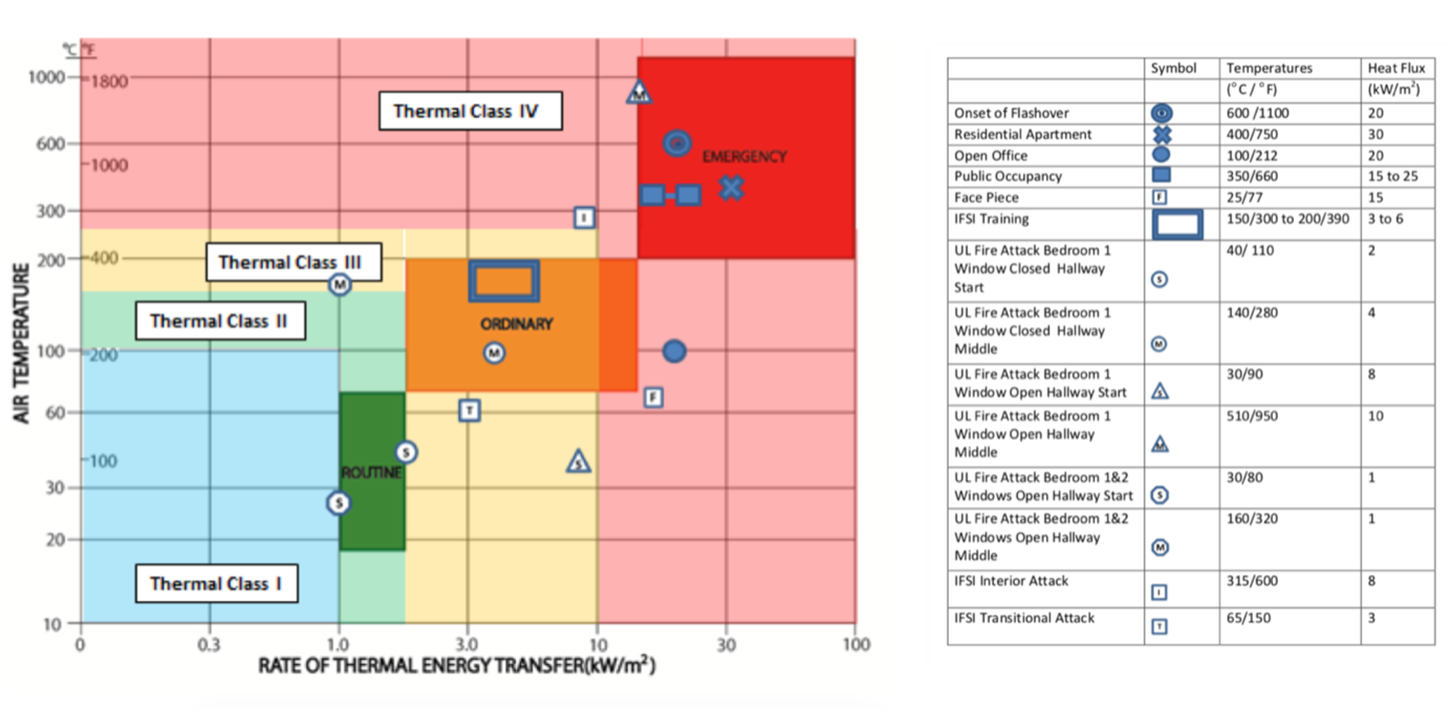
\includegraphics[width=0.9\textwidth]{Fig1_ThermalClass.png}
%\caption{. Thermal conditions potentially encountered during firefighting operations \cite{madrzykowski_fire_2017}.}\label{fig1}
%\end{figure}

Exposure of facepiece lenses to low intensity, repeat thermal loads (Routine and Ordinary conditions \cite{madrzykowski_fire_2017}) has been shown to have a negative impact on the mechanical properties of the SCBA facepiece \cite{horn_study_2017}. The appearance of thermal damage occurred after only 10 five-minute cycles at 5 kw/m\textsuperscript{2}. Mechanical properties were altered after 100 cycles of exposure, even in samples that did not include visible damage.  These experiments demonstrated that physical changes to the lens may occur during standard use and may not be immediately evident upon routine inspection of the facepiece lens. 

Building on the repeat exposure studies conducted by Horn, Kesler et al. \cite{horn_study_2017}, Kesler, Mistingas et al. \cite{kesler_mechanical_2018} examined the mechanical properties and thermal performance of new and field-utilized SCBA facepiece lenses. Sections of lenses were subjected to quasi-static tensile and impact tests, as well as to the “Lens Radiant Heat Test” in the 2013 edition of NFPA 1981 \cite{national_fire_protection_association_nfpa_2013}. Exposure to repeated thermal loads was shown to impact mechanical properties of the lenses, but no facepiece lenses failed to maintain positive pressure in the “Lens Radiant Heat Test”.  

Important questions still remain regarding the performance of SCBA facepiece lenses outside of the Routine and Ordinary condition exposures. Exposures classified as Thermal Class III and IV present serious hazardous to firefighters and may be encountered when fire conditions rapidly change and/or when firefighters become located in the exhaust portion of the fire flow path.

\subsection{Objectives}
The objectives of this study were to examine the thermal degradation of SCBA facepiece lenses during single exposures to heat flux values representative of fireground conditions. New, unexposed, facepiece lenses meeting both the 2007 and 2013 editions of NFPA 1981 were tested. Specifically, the following two metrics were examined under various heat fluxes:

\begin{itemize}
    \item{Thermal degradation of the facepiece as characterized by time to crazing, bubbling, and hole formation.}
    \item{Temperature at critical points within the SCBA facepiece.}
\end{itemize}


\section{Methods}\label{sec2}
\subsection{Materials}\label{subsec2}
Three models of SCBA facepieces were tested, all sourced from a single manufacturer and manufactured in May and June 2021. Facepieces met the standards laid forth in NFPA 1981, with two models following NFPA 1981 – 2007 edition and one model following NFPA 1981 – 2013 edition. The first model, \textbf{1-07A} meets the 2007 edition of NFPA 1981 and utilizes older construction and geometry, with hardware to attach the frame and harness passing through the lens. The second model, \textbf{1-07B}, also meets the 2007 edition of NFPA 1981 and features updated geometry where the frame and harness are attached by a clamp style closure around the edge of the mask. Lastly, the third facepiece model, \textbf{1-13}, meets the 2013 edition of NFPA 1981 and has similar geometry to 1-07B. The facepiece models are summarized in Table \ref{tab1} and are the same facepiece models as were utilized in a previous report \cite{kesler_mechanical_2018}. 

\begin{table}[h]
\begin{center}
%\begin{minipage}{174pt}
\caption{SCBA facepiece models utilized, similar to those used in a previous series of experiments \cite{kesler_mechanical_2018}.}\label{tab1}%
\begin{tabular}{rl}
\toprule
SCBA Facepiece & Description  \\
\midrule
107-A    & Meets NFPA 1981-2007 edition, older geometry   \\
107-B    & Meets NFPA 1981-2007 edition, updated geometry     \\
1-13    & Meets NFPA 1981-2013 edition  \\
\botrule
\end{tabular}
%\footnotetext{Source: This is an example of table footnote. This is an example of table footnote.}
%\footnotetext[1]{Example for a first table footnote. This is an example of table footnote.}
%\footnotetext[2]{Example for a second table footnote. This is an example of table footnote.}
%\end{minipage}
\end{center}
\end{table}

\subsection{Testing Apparatus}\label{subsec3}
%%

A natural gas fired radiant panel was utilized to provide consistent and repeatable thermal loads to the facepieces. Previous studies have utilized the same radiant panel \cite{horn_study_2017,kesler_mechanical_2018} based on the setup utilized by Putorti, Mensch et al.\cite{putorti_thermal_2013} and utilized in the “Lens Radiant Heat Test” from NFPA 1981 \cite{national_fire_protection_association_nfpa_2013}. An \mbox{air/gas} mixture provides a uniform flame across the 39 cm (15.4 in) tall by 33 cm (13.0 in) wide panel. Air is fed to the panel at a rate of 450 L/min and natural gas is supplied at 33 L/min. 

Prior to each test, the testing apparatus was allowed to run for one hour to ensure that steady state conditions were achieved. Immediately prior to each scenario, a water-cooled Schmidt-Boelter heat flux gauge (Medtherm Corp., Huntsville, AL, USA) was utilized to locate the prescribed heat flux. Heat flux was controlled by adjusting the distance between the gauge and the radiant panel along a linear track. After determining the proper location, the distance was marked, and the gauge removed from the test stand. At the highest heat flux, a minimum distance of 30cm (11.8in) was maintained between the panel and the facepiece to minimize convective heat transfer. 

Facepieces were positioned on a breathing headform, such that the surface of the lens was parallel to the radiant panel as in previous studies \cite{putorti_thermal_2013,horn_study_2017,kesler_mechanical_2018}. Components of the facepiece were protected with aluminum tape to avoid damage to the non-lens components with repeated testing. A Posi 3 USB PosiChek system (Honeywell, USA) was utilized to control the breathing headform. To align with NFPA 1981 \cite{national_fire_protection_association_nfpa_2013}, breathing was set to a rate of 40L/min. A standard fire service self-contained breathing apparatus was used to supply air to the headform. 

\subsection{Experimental Design}\label{subsec4}
Tests were conducted at four heat flux intensities representing a range of thermal classes. Heat fluxes of 5kW/m\textsuperscript{2}, 10kW/m\textsuperscript{2}, 15kW/m\textsuperscript{2}, and 20kW/m\textsuperscript{2} were selected as they range from ordinary to emergency thermal classes \cite{utech_status_1973}. Each facepiece lens was exposed to the prescribed heat flux until the lesser of 30 minutes or the occurrence of hole formation. At the end of the trial, the radiant load was removed, and breathing and data collection continued for two additional minutes. Three replicates of each condition were conducted. 

\subsection{Thermal Degradation}\label{subsec5}
Thermal degradation of the facepiece lenses was recorded throughout each of the tests. To quantify this metric, time to critical degrees of thermal degradation was recorded. Three degrees of degradation were tracked as in previous studies \cite{mensch_fire_2011}. Specifically, time to crazing, bubbling, and hole formation were recorded. Representative examples of thermal degradation are shown in Figure \ref{fig2}. Crazing and bubbling were tracked visually and verified with video recording of each test. Hole formation was also tracked visually and verified by a change in pressure as recorded by the PosiChek between the inside surface of the lens and the headform. 

\begin{figure}[h]%
\centering
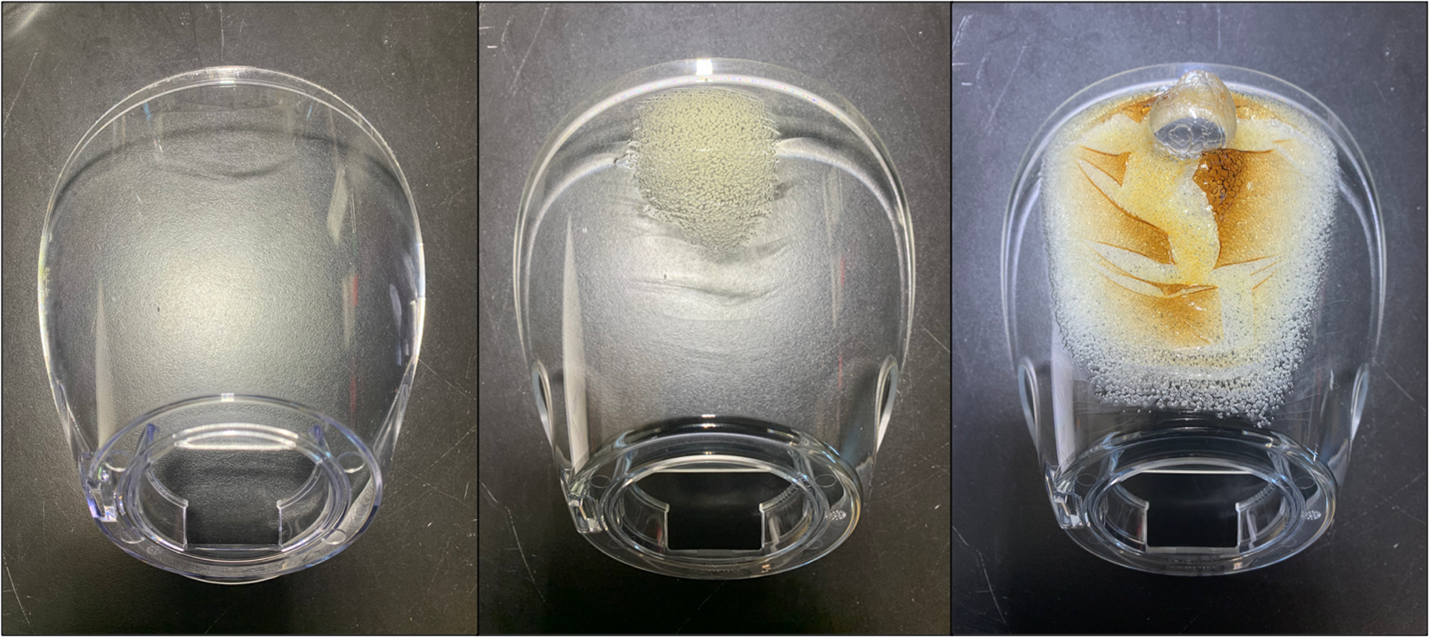
\includegraphics[width=0.9\textwidth]{Fig2_ThermalDeg.png}
\caption{. Representative images of thermal degradation: crazing (left), bubbling (center), and hole formation (right).}\label{fig2}
\end{figure}

\subsection{Temperature Logging}\label{subsec6}
Throughout each test, temperature was recorded at two locations. Inspired air temperature was recorded at the airway (Location 1) and the inside air temperature was measured between the inside surface of the lens and the headform (Location 2, Figure \ref{fig3}). Data were collected at 1 Hz, using Nickel-Chromium / Nickel-Alumel Type K thermocouples secured with aluminum tape. Data were recorded with a Squirrel 2040 Series Data Logger (Grant Instruments, Beaver Falls, PA, USA).

\begin{figure}[h]%
\centering
\includegraphics[width=0.9\textwidth]{Fig3_Temp.png}
\caption{. Thermocouple locations. Temperature was measured at the airway (Location 1, left) and the dead space between the lens and headform (Location 2, right).}\label{fig3}
\end{figure}

\subsection{Data Analysis}\label{subsec7}
Time to thermal damage was averaged across three replicate trials for all conditions. In some instances, the lens did not reach specific damage thresholds within the 30-minute test. Maximum temperature was calculated as the highest temperature reached throughout the trial. Replicate trials were averaged across three trials except in the case of condition 1-13 at 10kW/m\textsuperscript{2} in which only two replicates had usable temperature data. Paired t-tests were conducted for time to thermal damage and temperature data, with the results determined to be statistically significant when p-value\textless 0.05.{}

\section{Results and Discussion}\label{sec3}
\subsection{Themal Degradation}\label{subsec7}
Time to thermal degradation was recorded and is reported in minutes to time of event (Table \ref{tab2}). In some instances, certain thresholds of thermal degradation did not occur within the 30-minute test. These instances are noted with “--” in Table \ref{tab2}. 


\begin{table}[h!]
\begin{center}

\caption{Time to thermal degradation by mask type and heat flux. All times reported as mean (SD) in minutes (min). \textsuperscript{†}indicates significant difference between 1-07A and 1-07B. *indicates that 1-13 is significantly different from 1-07A and 107B.}\label{tab2}

    \begin{tabular}{lccccc}
      \toprule
      \textbf{Damage} & \textbf{Facepiece} & $\textbf{5 kW/m\textsuperscript{2}}$ & $\textbf{10 kW/m\textsuperscript{2}}$ & $\textbf{15 kW/m\textsuperscript{2}}$& $\textbf{20 kW/m\textsuperscript{2}}$\\
      \botrule
      & 1-07A & 19.3 (1.2)\textsuperscript{†} & 1.3 (0.3) & 0.7 (0.1) & 0.5 (0.1)\\ 
      \cmidrule{2-6}
      Crazing & 1-07B & 8.3 (1.9) & 1.3 (0.1) & 0.9 (0.2) & 0.7 (0.2)\\ 
      \cmidrule{2-6}
      & 1-13 & -- & 3.8 (0.5)* & 1.7 (0.1)* & 1.1 (0.1)*\\ 
      \botrule

        & 1-07A & -- & 2.6 (0.2) & 1.2 (0.1) & 0.9 (0.0)\\ 
      \cmidrule{2-6}
      Bubbling & 1-07B & -- & 2.3 (0.0) & 1.4 (0.1) & 0.9 (0.0)\\ 
      \cmidrule{2-6}
      & 1-13 & -- & 8.2 (2.1)* & 2.6 (0.2)* & 1.6 (0.0)*\\ 
      \botrule

        & 1-07A & -- & -- & 4.7 (2.9) & 1.8 (0.1)\\ 
      \cmidrule{2-6}
      Hole Formation & 1-07B & -- & 13.4 (4.3) & 3.2 (0.6) & 1.9 (0.1)\\ 
      \cmidrule{2-6}
      & 1-13 & -- & -- & -- & 7.0 (0.7)*\\ 
      \botrule
     
    \end{tabular}
  
  \end{center}
\end{table}

At 5 kW/m\textsuperscript{2}, 1-07A and 1-07B had statistically significant differences in time to crazing, with damage appearing in 1-07B over twice as fast as in 1-07A. None of the facepiece lenses tested developed hole formation or bubbling at 5 kW/m\textsuperscript{2}. Putorti et al. did report two facepiece lens models showing bubbling at 5 kW/m\textsuperscript{2}, but our results are consistent with the reported results for hole formation \cite{putorti_thermal_2013}. 

At 10 kW/m\textsuperscript{2}, all lenses showed crazing and then developed bubbling. No significant differences were observed in time to bubbling or crazing between 1-07A and 1-07B, though 1-13 took significantly longer to develop either sign of thermal degradation. 1-07B developed hole formation at 13.4 minutes, slightly longer than previous work has observed in facepieces held to a similar standard \cite{putorti_thermal_2013}, but hole formation was not observed in 1-07A or 1-13.

At 15 kW/m\textsuperscript{2}, 1-13 developed crazing and bubbling significantly slower than either 1-07A or 1-07B and did not develop a hole throughout the 30-minute test. There were no statistically significant differences between 1-07A and 1-07B for any of the levels of thermal degradation. The times for 1-07A and 1-07B align very closely with the previous literature \cite{putorti_thermal_2013}. The increased time to thermal degradation in the 1-13 lenses shows the impact of the changes in facepiece lens construction as a result of the introduction of the “Lens Radiant Heat Test” from NFPA 1981 \cite{national_fire_protection_association_nfpa_2013}.

At 20 kW/m\textsuperscript{2}, all facepiece lenses reached hole formation. 1-07A and 1-07B lenses developed crazing in just 31 and 42 seconds respectively (though not statistically different), bubbling occurred in under 1 minute, and holes developed after less than two minutes of exposure. The 1 13 lenses had significantly longer times to thermal degradation for each metric. Again, these results indicate that masks which are compliant to the “Lens Radiant Heat Test” will result in longer times to degradation than those lenses designed to meet older editions of the standard without the “Lens Radiant Heat Test”.

\subsection{Temperature}\label{subsec8}
At the lowest heat flux intensity (5 kW/m\textsuperscript{2}) temperatures at Location 1 and 2 were not statistically significant from each other.  At 10 kW/m\textsuperscript{2} temperatures at the headform were not significantly different between 1-07A and 1-13, but there were significant differences between 1-07A and 1-07B, and nearly significant differences between 1-07B and 1-13 (p=0.081). For tests at 15 and 20 kW/m\textsuperscript{2}, 1-13 reaches significantly higher temperatures at both locations (Table \ref{tab3}). This can likely be attributed to the duration of the exposure, as the 1-13 lenses took significantly longer to reach hole formation. The higher temperatures may be critical to a firefighter wearing the SCBA, as even though the mask may not develop a hole, the temperatures may not be sustainable without potential injury.

\begin{table}[h!]
\begin{center}

\caption{Maximum temperature in the airway and the air between the lens and headform. Data are presented as mean (SD) in degrees Celsius.}\label{tab3}

    \begin{tabular}{lccccc}
      \toprule
      \textbf{Location} & \textbf{Facepiece} & $\textbf{5 kW/m\textsuperscript{2}}$ & $\textbf{10 kW/m\textsuperscript{2}}$ & $\textbf{15 kW/m\textsuperscript{2}}$& $\textbf{20 kW/m\textsuperscript{2}}$\\
      \botrule
      & 1-07A & 56.8 (3.9) & 82.2 (3.0) & 56.9 (9.1) & 50.1 (4.6)\\ 
      \cmidrule{2-6}
      Airway & 1-07B & 59.0 (4.2) & 69.6 (6.0) & 51.4 (7.2) & 50.0 (0.6)\\ 
      \cmidrule{2-6}
      & 1-13 & 58.2 (5.9) & 81.3 (1.5) & 95.4 (2.1) & 72.6 (5.2)\\ 
      \botrule

        & 1-07A & 82.4 (6.1) & 123.1 (13.7) & 95.2 (15.5) & 98.9 (10.1)\\ 
      \cmidrule{2-6}
      Dead Space & 1-07B & 84.6 (3.8) & 104.1 (10.0) & 88.5 (9.0) & 85.6 (8.4)\\ 
      \cmidrule{2-6}
      & 1-13 & 84.4 (9.7) & 112.2 (7.0) & 130.1 (2.8) & 111.0 (2.5) \\ 
      \botrule


     
    \end{tabular}
  
  \end{center}
\end{table}

\section{Conclusion}
Previous research has shown the SCBA facepiece to be susceptible to damage from thermal loads which can be encountered during firefighting operations. This work has led to changes to NFPA 1981, specifically the introduction of the “Lens Radiant Heat Test” \cite{national_fire_protection_association_nfpa_2013}. SCBA facepieces meeting the 2013 edition of NFPA 1981 had increased time to thermal degradation and avoided hole formation at all but the most extreme heat flux tested (20 kW/m\textsuperscript{2}). Maximum temperature within these facepiece lenses was higher than those meeting older editions of the standard, likely due to longer exposure times. 

As in previous research, thermal loads are applied from a flat panel and directed to the parallel lens surface. This limitation does not fully reflect the radiant loads under fire conditions which may reach the facepiece from multiple sources. Further, changes in the environment firefighters operate in (increased fuel loads, higher heat release rates) as well as advances in other areas of personal protective equipment, drive the need for further research into thermal degradation of facepiece lenses. 


\section*{Declarations}
\subsection*{Funding}

This project was funded as part of a subaward agreement to the Illinois Fire Service Institute through Underwriter Laboratories’ Fire Safety Research Institute under DHS FEMA Assistance to Firefighter Grant EMW-2018-FP-00476. 


% \begin{itemize}
% \item Funding
% \item Conflict of interest/Competing interests (check journal-specific guidelines for which heading to use)
% \item Ethics approval 
% \item Consent to participate
% \item Consent for publication
% \item Availability of data and materials
% \item Code availability 
% \item Authors' contributions
% \end{itemize}

% \noindent
% If any of the sections are not relevant to your manuscript, please include the heading and write `Not applicable' for that section. 

%%===================================================%%
%% For presentation purpose, we have included        %%
%% \bigskip command. please ignore this.             %%
%%===================================================%%
% \bigskip
% \begin{flushleft}%
% Editorial Policies for:

% \bigskip\noindent
% Springer journals and proceedings: \url{https://www.springer.com/gp/editorial-policies}

% \bigskip\noindent
% Nature Portfolio journals: \url{https://www.nature.com/nature-research/editorial-policies}

% \bigskip\noindent
% \textit{Scientific Reports}: \url{https://www.nature.com/srep/journal-policies/editorial-policies}

% \bigskip\noindent
% BMC journals: \url{https://www.biomedcentral.com/getpublished/editorial-policies}
% \end{flushleft}

%%===========================================================================================%%
%% If you are submitting to one of the Nature Portfolio journals, using the eJP submission   %%
%% system, please include the references within the manuscript file itself. You may do this  %%
%% by copying the reference list from your .bbl file, paste it into the main manuscript .tex %%
%% file, and delete the associated \verb+\bibliography+ commands.                            %%
%%===========================================================================================%%

%%\bibliography{sn-bibliography}% common bib file
\bibliography{SCBA_ThermalDegradation.bib}% common bib file
%% if required, the content of .bbl file can be included here once bbl is generated
%%\input sn-article.bbl

%% Default %%
%%\input sn-sample-bib.tex%

\end{document}
